\documentclass[12pt,a4paper]{article} 

\usepackage[utf8]{inputenc}  %% UTF-8 encoding
\usepackage[british,UKenglish]{babel}  %% Language
\usepackage[a4paper, margin=1in]{geometry} %% margins
\usepackage{graphicx}
\usepackage[export]{adjustbox}
\usepackage[absolute,overlay]{textpos}
\usepackage{tikz}
\usepackage{algorithm}
\usepackage{algpseudocode}  %% Only use algpseudocode, not algorithmic
\usepackage{amsmath,amsfonts,amssymb}
\usepackage{lastpage}
\usepackage[round,authoryear]{natbib}  %% Harvard-style citations
\usepackage[bookmarks=true, colorlinks=true, linkcolor=blue, citecolor=black, urlcolor=blue]{hyperref}
\usepackage{booktabs} % Better tables
\usepackage{array} % Enhanced table formatting
\usepackage{textcomp} % For text symbols
\usepackage{breakurl} 

% Unicode character definitions
\DeclareUnicodeCharacter{03BB}{$\lambda$}  % Greek lambda
\DeclareUnicodeCharacter{2713}{\checkmark}  % Checkmark

% Bibliography configuration for Harvard style
\bibliographystyle{agsm}  % Harvard style (Author-Year)


\DeclareGraphicsExtensions{.pdf,.png,.jpg}
\graphicspath{{./figures/}}

\newcommand{\mytype}{MSc Research Project}
\newcommand{\mystream}{Cybersecurity}


\newcommand{\myname}{Soukya Koleti}
\newcommand{\studentID}{23214490}
\newcommand{\mytitle}{Adversarial Robustness of Deep Residual Learning for Audio Spoofing Detection in Automatic Speaker Verification Systems}

\newcommand{\wordcount}{3000} 

\newcommand{\supervisor}{Mosab Mohamed}
% \newcommand{\supervisortwo}{XXX} 

\newcommand{\myyear}{2025}
\newcommand{\duedate}{14/12/2025}

\hypersetup{
 pdfauthor={\myname},
 pdftitle={\mytitle},
 pdfsubject={\mytype},
 pdfkeywords={\mystream}
} 

\setlength{\marginparwidth}{20mm}

\newcommand{\margtodo}
{\marginpar{\textbf{\textcolor{red}{ToDo}}}{}}

\newcommand{\todo}[1]
{{\textbf{\textcolor{red}{(\margtodo{}#1)}}}{}}

% Describe separation hints here:
\hyphenation{
} 


\begin{document}

% \include{titlepage}
% \include{declaration} 

\title{\mytitle}%
%\author{\myname \\ \studentID \\ \mytype\ in \mystream}%
\author{\myname \\ \studentID}%
\date{}
\maketitle

\pagestyle{plain}
\pagenumbering{arabic}

\begin{abstract}
This work investigates the vulnerability of lightweight compact neural networks to voice spoofing via synthetic audio in the speaker verification task. Although deep neural architectures are predominant in modern detection systems and attain high performance, their heavy computational cost makes them impractical for pervasive devices like smartphones and smart speakers. To assess the viability of more lightweight models, we investigate a compact network with around 300K parameters under stringent adversarial conditions on two benchmark datasets: ASVspoof2019 LA and WILD. A mixed performance landscape is reflected in the results. The non-adversarial settings yielded an accuracy of 97.12\% for ASVspoof2019 LA and 99.38\% for WILD, which are respectable results. However, under controlled adversarial perturbations, the same model showed remarkable vulnerability: a FGSM perturbation of $\epsilon$=1.0 decreases accuracy by almost 50\% and increases the error rate by a factor of 17. For larger perturbation sizes, a strong PGD attack degrades accuracy to 10.2\% and 3.0\%. In comparing these with larger CNN architectures, although larger models are resistant to weak attacks, no architecture preserves robustness in an aggressive adversarial condition. A defensive training degrades the clean performance further-from 97.1\% to 85\% accuracy-without mitigating the underlying vulnerability. Taken together, the findings above suggest that efficient lightweight models intrinsically trade off security against efficiency, and existing defenses are too weak to address this trade-off effectively.
\end{abstract}


\section{Introduction}


\subsection{Background and Motivation}

From voice-unlocking your phone to issuing voice commands for a bank transfer, speaker verification has become part of everyday life. The idea is to identify your voice pattern from stored profiles, and for the most part, it works seamlessly. There is a catch, though: bad actors have found ways to dupe these systems using synthetic voices, converted speech patterns, or simple recordings. As today's text-to-speech tools get remarkably good at mimicking human voices, this threat keeps growing.

Meanwhile, detection systems invented by researchers try to find the fakes. The ASVspoof competition has helped move the field along by providing common benchmarks that different approaches can be compared against. The best-performing detectors tend to rely either on deep convolutional networks or sophisticated self-supervised learning setups; they work remarkably well in tests but have a problem: they require serious computing horsepower. That rules them out for smartphones, voice assistants, and other gadgets where battery life and/or processing speed is crucial.

The practical workaround has been simpler models: basic neural networks fed with log-mel spectrograms, running fast on limited hardware. But here is the question nobody has really answered: can those stripped-down detectors handle deliberate attacks? We know that carefully crafted input perturbations can break sophisticated deep learning models. What we do not know is how much worse the problem gets when the detector itself is lightweight.

\subsection{Research Gap}

Previous work on adversarial attacks against spoofing detectors (Liu et al., 2019; Wu et al., 2020) examined deep CNN architectures with millions of parameters. Nobody has done the same systematic testing on the simpler models that actually get deployed on phones and smart speakers. That gap matters because these compact architectures might behave quite differently under attack—they could be more fragile, surprisingly resilient,
or fail in unexpected ways. We simply do not know. On top of that, most testing happens on clean benchmark data like ASVspoof, which looks nothing like messy realworld recordings with background chatter, compression artifacts, and varying microphone quality

\subsection{Research Questions and Objectives}

The big-picture question driving this work: how vulnerable are lightweight spoofing detectors to adversarial attacks, and how do they stack up against beefier CNN architectures?

Breaking that down into testable pieces:

\begin{enumerate}
    \item How vulnerable are lightweight log-mel feedforward classifiers to white-box adversarial attacks (FGSM and PGD) across varying perturbation strengths ($\epsilon$ = 0.1, 1.0, 5.0)?
    
    \item Does adversarial susceptibility differ between controlled benchmark datasets (ASVspoof2019 LA) and realistic unconstrained datasets (WILD) when using identical lightweight architectures?
    
    \item How do the robustness characteristics of lightweight models compare with CNN-based architectures (LCNN, SENet) under equivalent attack conditions?
    
    \item How do adversarially perturbed images affect the metrics of total performance (Accuracy) as well as the following metrics: Equal Error Rate (EER); False Acceptance Rate (FAR); False Rejection Rate (FRR) and Attack Success Rate for both datasets?
\end{enumerate}

To answer these questions, the research tackles six concrete objectives:

\begin{enumerate}
    \item \textbf{Baseline Validation:} Reproduce the adversarial robustness experiments with CNNs in Liu et al. (2019) using both LCNN and SENet architectures to establish valid baselines and verify that their attack implementation is correct.
    
    \item \textbf{Lightweight Model Development:} Develop and train a resource-efficient feedforward spoofing detector ($\sim$300K  parameters) using log-mel spectrograms, with optimization aimed at the deployment of models on mobile and embedded devices.
    
    \item \textbf{Adversarial Vulnerability Assessment:} Systematic evaluation of lightweight model robustness under the FGSM and PGD white-box attacks is conducted using three perturbation magnitudes, $\epsilon$ = 0.1, 1.0, 5.0, on ASVspoof2019 LA and WILD.
    
    \item \textbf{Comparative Architecture Analysis:} Variances in the robustness of both lightweight feedforward networks and high-capacity CNN architectures are quantified to identify architecture-specific vulnerability patterns.
    
    \item \textbf{Defense Mechanism Evaluation:} Assess how well adversarial training serves as a defense mechanism for lightweight models. Analyze capacity–robustness trade-off.
    
    \item \textbf{Practical Deployment Implications:} Critically discuss security trade-offs, deployment constraints, and recommend alternative defense strategies for resource-constrained automatic speaker verification systems.
\end{enumerate}

\subsection{What This Work Contributes}

The main contribution of this work is to provide empirical evidence that lightweight spoofing detectors have a fundamentally different security profile than their larger counterparts. Concretely, this study shows: (1) this is the first systematic adversarial assessment of compact feedforward architectures for spoof detection; (2) an identified capacity–robustness trade-off prevents sub-500K-parameter models from achieving both robust clean performance and adversarial robustness under standard defenses; (3) the reproducibility framework introduced allows for apples-to-apples comparisons across various architectures; and (4) the described vulnerability patterns are consistent under both the ASVspoof and WILD datasets.

\subsection{Assumptions and Scope}

The following are a set of considerations that guided this study: An attacker is assumed to have complete access to the model, including its architecture and weights. This is the worst-case scenario because a model under these conditions, if it does not hold up, will not be able to hold up against more realistic threat models. The analysis is focused on the feature domain (specifically log-mel spectrograms) and not on raw audio waveforms. This allows the classifier to be separated from any potential complexity in the signal processing. The types of attacks that were analysed were restricted to FGSM and PGD attacks. Although other techniques exist, these are the two that are considered standard methods in the gradient-based attack family. Finally, the study is limited to binary true-vs-fake classification, and therefore does not cover other multi-class identification methods or attacks that involve joint speaker verification.

\subsection{Report Structure}

This report consists of a review of prior research (Section 2), the design of our experiments-the tools we used and the way we conducted them (Section 3), how to build a new version of WhatWeAre using machine learning (Section 4), how to create a working version of WhatWeAre (i.e. the hardware, software, and Web interfaces) (Section 5), how to evaluate our machine-learning system for predicting poets’’ popularity (and other factors) (Section 6), what the findings of our research suggest and what they don’t (Section 7), and what this means for the future and beyond (Section 8).


\section{Literature Review}

In this chapter, we will examine the evolution of both spoofed attacks and socalled "defense technology" against such attacks. We will examine how the movement from the image-based world to the audio-based adversarial environment changed the types of attacks and defenses as well. Next, we will review the weaknesses of the currently employed imitation ("disguised") defense mechanisms against spoofed attacks. Finally, we will identify the gap of not researching the use of lightweight models in this area.

\subsection{Evolution of Spoofing Attacks and Countermeasures}

For more than ten years, spoofing and detection have existed in a cat-and-mouse relationship. The early detection methods were based on extracting audio characteristics manually (MFCCs or CQCCs) and trained using traditional machine learning algorithms (GMMs or SVMs). These methods were effective at detecting spoofing, but they became ineffective because the adversaries developed their capabilities. In 2015, ASVspoof began creating a standard metric to evaluate systems. In 2019 the metrics were raised to include TTS and voice conversion attack methods which many of the traditional systems failed to perform effectively.

This transition took place with the introduction of deep learning. Convolutional neural networks processing spectrogram representations directly started to outperform manually tuned techniques; notably, the LCNN and SENet architectures brought significant improvements in detection accuracy. Very recently, self-supervised learning paradigms have also shown promising potential. A common weakness of these top-performing methods is their high computational and parameter costs: many models have millions of parameters and require significant processing resources. This creates a major barrier to using these methods on resource-constrained devices like mobile phones and smart speakers. Thus, lighter-weight methods, such as shallow networks and simpler feature representations, continue to see deployment despite open questions about their security properties.

\subsection{Adversarial Attacks in Audio Domains}

This alert originated from visual-domain findings. In 2013, studies demonstrated that imperceptible perturbations added to an image could induce neural networks to misclassify with high confidence, with this adversarial effect frequently transferring across distinct models. The implication was that analogous vulnerabilities might be exploited within the audio modality. In 2018, Carlini and Wagner showed that speech recognition systems could be manipulated to recognize arbitrary target content chosen by an attacker.

Test Cases. Liu et al. (2019) conducted rigorous testing of spoofing detectors via two different attack strategies—one based on FGSM (Fast Gradient Sign Method)—which was quick to develop but was ultimately heuristic and limited; while the other, PGD (Projected Gradient Descent)—which has proven to be an effective and stronger threat, with significantly greater computational requirements than the FGSM method. Results showed that when faced with adversarial threats, spoofing detector performance declined dramatically, with a large percentage of detectors having drop rates below 20\% when subjected to such threats, despite being able to achieve 95\% accuracy on clean audio. Interestingly, black-box attack techniques, which allow an attacker to attack a model without having any insight into the internals of that model, continue to be effective. Since that time, the issues identified during the Liu et al. (2019) study have continued into the 2023-2024 timeframe and have generated reports of increased error rates in subsequent follow-up studies of at least 40\% (compared to the previous ranges of 7\% to 9\% for example); one publication indicated that accuracy for the same detector went from 98.5\% to 0.08\% due to being attacked.

\subsection{Defense Mechanisms and Limitations}

Before long, researchers recognized that adversarial examples could be used in the same way that traditional attacks could be utilized against an algorithm. At that point, researchers turned their attention towards developing methods to mitigate the impact of adversarial examples on their algorithms. This led to two distinct classes of approaches used to deal with adversarial examples: pro-active methods and re-active methods. Pro-active approaches aim to create a model that is more robust by employing techniques from the adversarial training literature and adopting a focused approach to adversarial training in developing a model. In a study published by Wu et al. (2020) where the study applied the adversarial training methodology to its models, the study showed an increase in accuracy from only ~15\% to ~30\% which is an improvement, but clearly not adequate for a mission critical operation. In contrast, re-active methods attempt to mitigate the effect of adversarial examples by "cleaning" the input data of adversarial examples before presenting them to the model, which can be accomplished by either applying smoothing to the input or performing feature transformation to the data before presenting it to the model.

Researchers have a challenge determining which approach works best for them to get the highest performance. Adversarial training can be time-consuming and lead to lower accuracies on "standard" training datasets due to the time being spent on processing adversarial input samples when running the algorithm. The input preprocessing may also take out any valid inputs leading to missing data within the datasets. And, the defense mechanisms that protect against certain classes of adversarial attacks will often not help to protect against other classes of attacks. For instance, for lightweight models, adding on additional layers of defense will create an increase in the model size making it counterproductive to develop lightweight machine learning solutions.

\subsection{The Lightweight Model Gap}

Adversarial robustness research has focused on big models (for instance Liu et al.'s work with LCNN and SENet and Wu et al.'s use of similar sized architectures), & more recently some work in the self-supervised field has also examined networks with tens of millions of parameters. In contrast, smaller networks that run on consumer hardware (e.g., simple feedforward MLPs and basic classifiers) have not been commonly tested for security. Because these smaller architectures can have limited capacity to learn robust feature representations, they might be especially susceptible to adversarial attacks or conversely they may be less so because their smaller size results in a lower attack surface area. Other, potentially different, factors may be relevant, but without experimental testing, it is impossible to verify.

\subsection{Summary and Research Justification}

This indicates that much progress has been made regarding the detection of spoofing attempts and understanding the ways in which attackers exploit heavyweight models, but there are still many security issues regarding lightweight systems. We have closed this gap through a systematic application of stress-testing procedures on compact feedforward networks (CFNs), providing performance benchmarks relative to standard convolutional neural networks (CNNs) and interpreting results within the context of practical use scenarios.

\section{Methodology}

This section specifies how the experiments were conducted - in sufficient detail for anyone to repeat them and the processes were identical from dataset handling to generating attacks. 

\subsection{Research Design Overview}

To compare the different models - lightweight model and CNN model - a side-by-side comparison used the same processing chain on each of the two datasets, ASVspoof2019 LA (which represents a clean benchmark scenario) and WILD (consisting of real-world noisy audio). The processing workflows were identical for both families of models, using the same extraction of features (log-mel) and training of classifiers, and then both sets of models were subjected to a series of attacks at various intensities using FGSM and PGD adversarial examples. By doing so, the original CNN experiments conducted by Liu et al. (2019) can be used as a reference point for verification of the accuracy of the approach used to produce the attacks and the baseline CNN performance can be established for comparison with the lightweight models and any differences in performance will be related to the respective model architectures instead of any unique configuration characteristics associated with the experiment setup.

Figure: \ref{fig:system_architecture} Overall system architecture and experimental pipeline, which present the parallel processing sequence for both ASVspoof and WILD datasets, through feature extraction to model training, and finally, adversarial evaluation.

\begin{figure}[h]
\centering
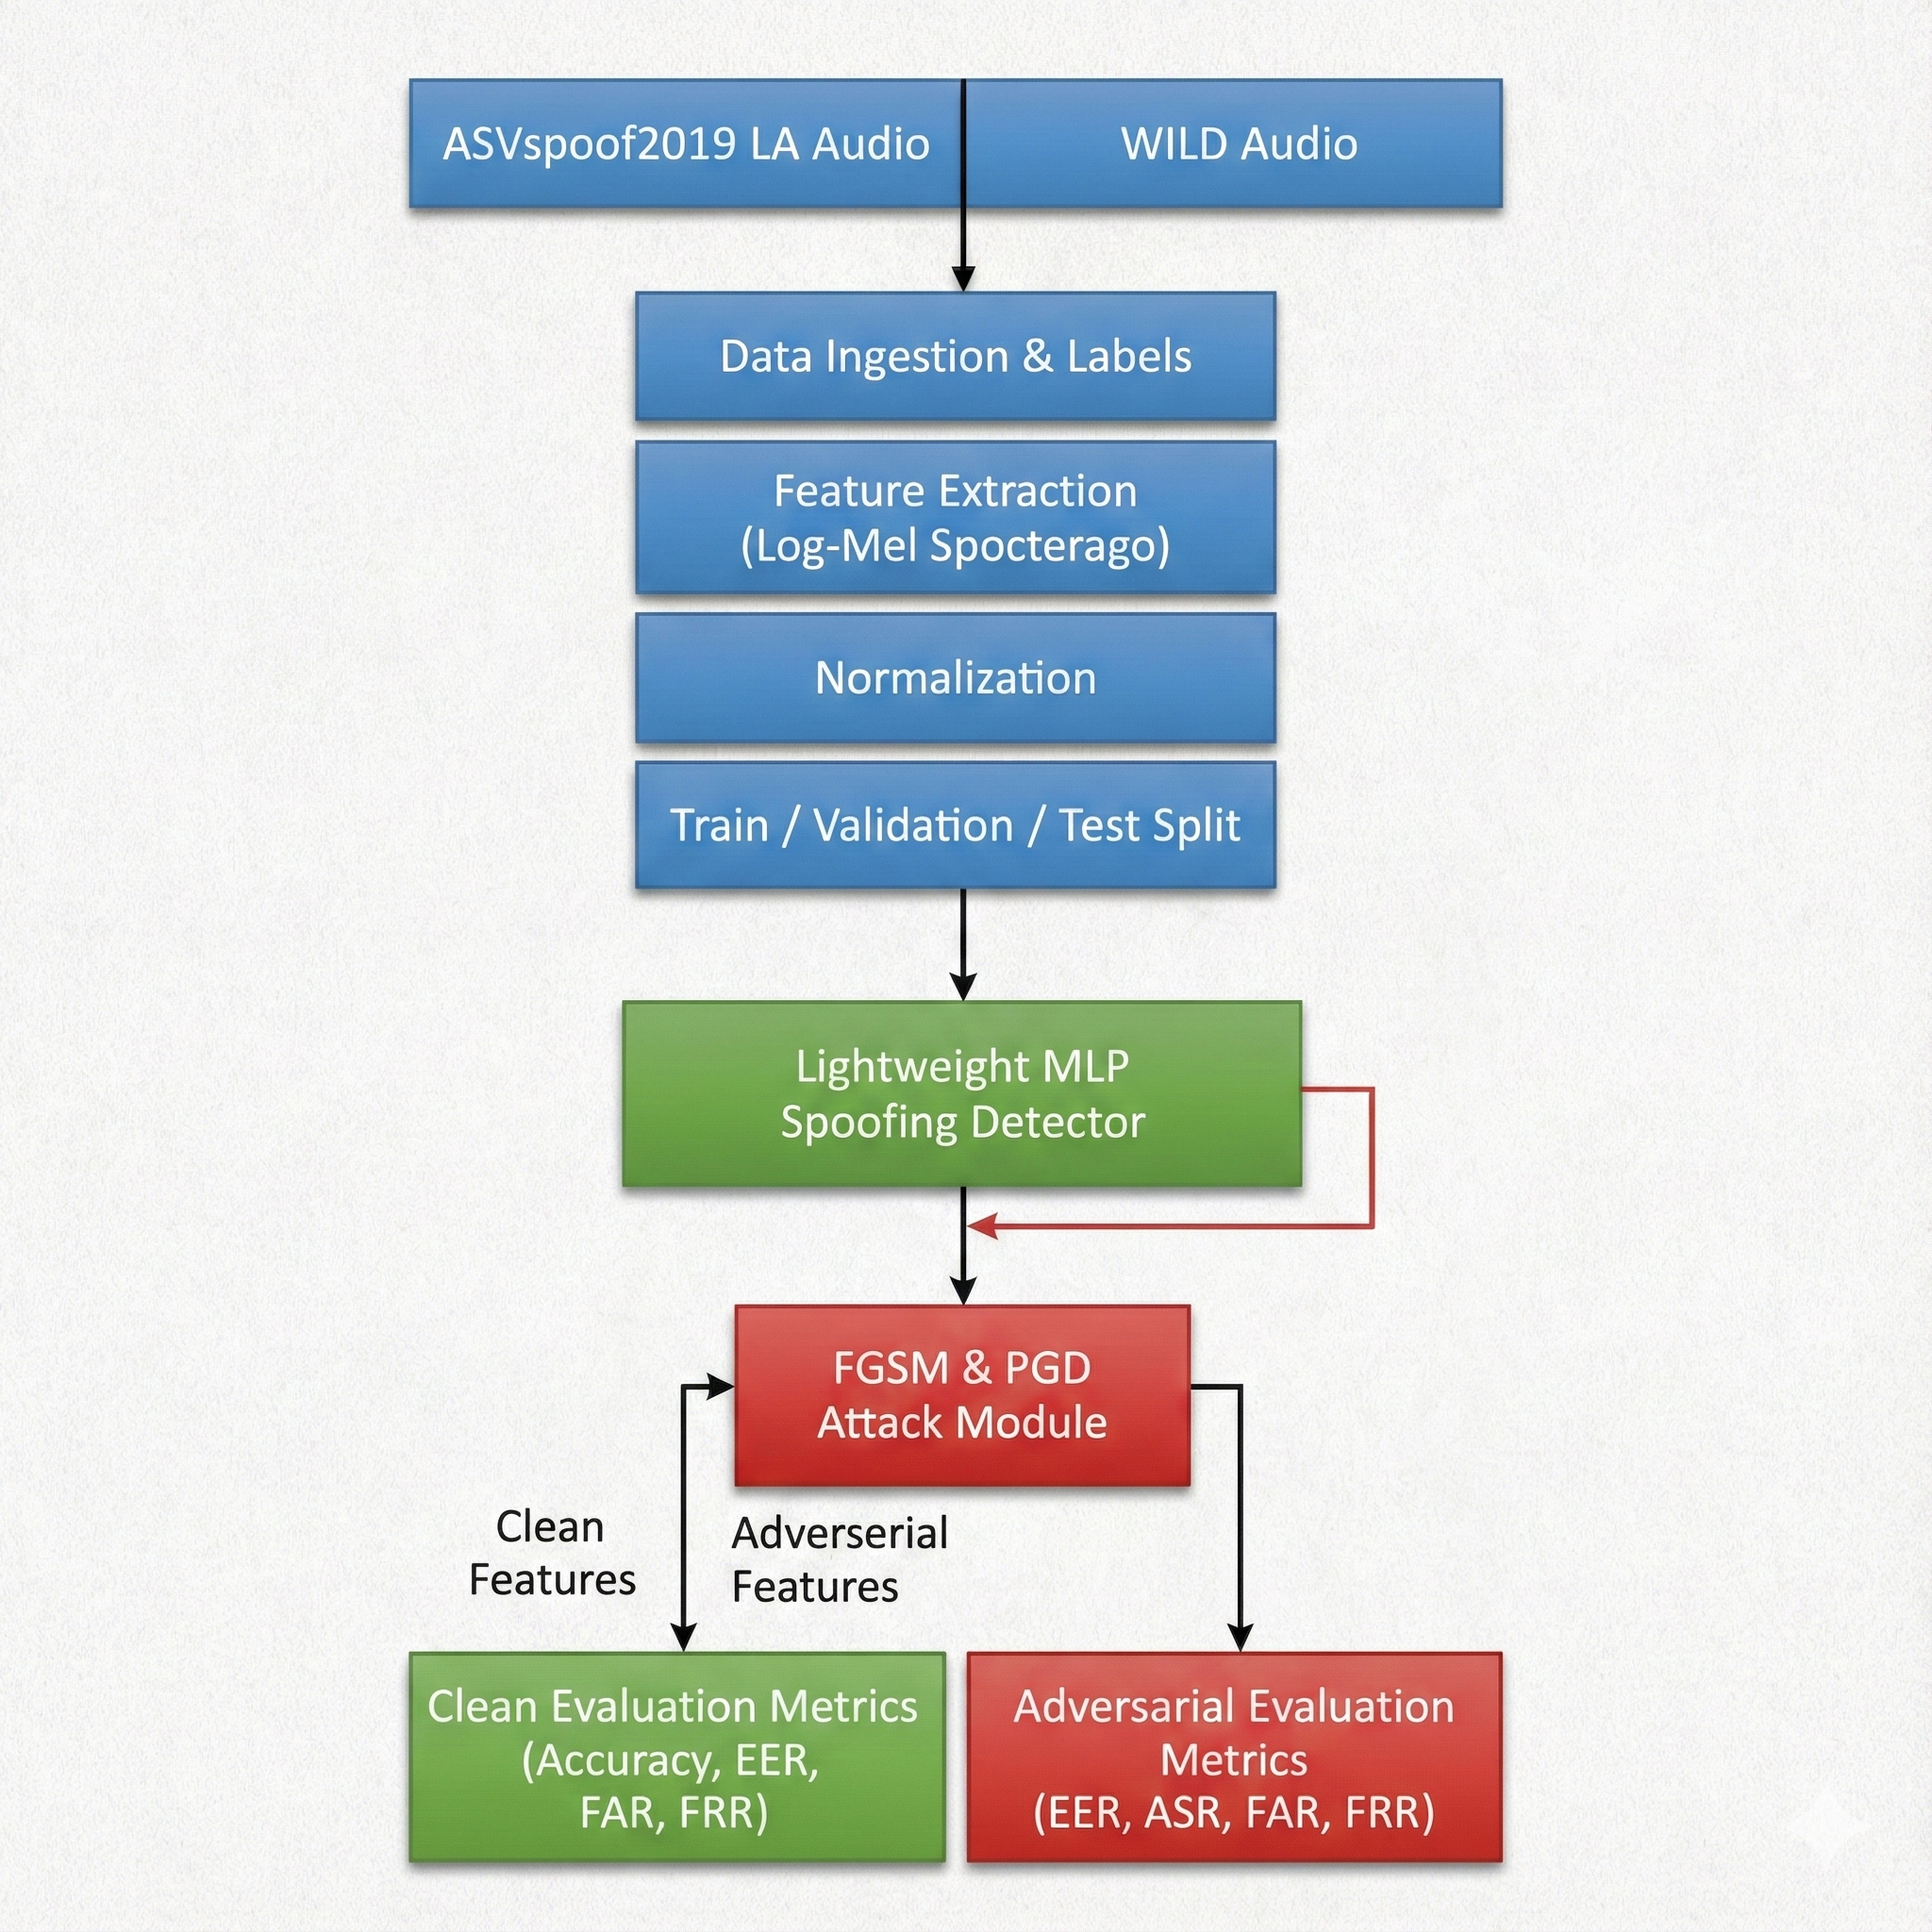
\includegraphics[width=0.95\textwidth]{figures/architecture_diagram.png}
\caption{System Architecture}
\label{fig:system_architecture}
\end{figure}

\subsection{Dataset Preparation}

\subsubsection{ASVspoof2019 LA Dataset}

The ASVspoof2019 Logical Access Dataset is an important benchmark in the area of detection of synthetic speech. In all, over 100,000 utterances were collected, which contain both authentic voices and many different types of synthetic attacks created with many different text-to-speech and voice conversion systems. The quality of this dataset comes from the fact that it was collected under controlled conditions and the types of attacks have been carefully documented. The ASVspoof2019 Logical Access dataset also has been assigned an official evaluation protocol, allowing for the comparison of results across all studies using this dataset.

Although this dataset has been extracted, it is important to handle these features with care. The extracted features exist in NumPy format, and each ID's array size is determined by the length of the associated utterance. These features were then transformed into a fixed-length vector of equal size for use with the feedforward neural network. This transformation process involved flattening the spectrogram of the time-frequency domain into a single vector, and then using either padding or truncation to achieve a constant vector size. Since this approach does not preserve the temporal structure of the data, the purpose of this method was to create a lightweight model focused on simplifying the complexity of the model.

The labels were defined clearly: 0 for true speech and 1 for impersonation. The same official training, development, and evaluation splits were used as the ones used in previous research on the same dataset. One of the biggest challenges faced when working with this dataset was that the class distribution was heavily skewed; the number of examples of impersonation was substantially larger than the number of examples of true speech cases. Because of this imbalance in the class distribution, it was necessary to utilize the weighted loss function approach as explained in section 3.3.1.

\subsubsection{WILD Dataset}

The developmental nature of the WILD dataset creates a unique set of difficulties, as it contains only raw audio waveform data (without any feature extraction) and is designed to reflect actual recording conditions that cannot be controlled. There are two folders in the WILD dataset for real and synthetic speech recordings, but there is no 'standard' protocol file, which means that a separate metadata structure must be created for each recording.

Waveform data was loaded into the preprocessing pipeline and resampled onto the regular 16 kHz sampling rate. To calculate log-mel spectrograms, librosa's library was used, with 80 mel bins being chosen as a good compromise between frequency resolution and compute time. After this step was finished, each spectrogram was converted to a decibel scale and normalized so that they all had a mean of 0 and variance of 1.

The issue of variability in length is exacerbated by the fact that recordings have been acquired from multiple sources that differ in length. As such, a single fixed length has been established for all of the spectrograms based upon the median length of all the recordings within the entire dataset; shorter recordings have been padded with zeros at the end, while longer recordings have been truncated. Even though truncating longer recordings could remove important components of the signal, flattening spectrograms into vectors allows for the consistent creation of batches for training, as well as consistency with the typical ASVspoof processing convention used during all experimental runs.

\subsection{Model Architecture}

\subsubsection{Lightweight Feedforward Classifier}

The lightweight model uses three hidden layers (512, 256, 64 units), ReLU activation, batch normalization, and 50\% dropout; thus, it contains approximately 300,000 parameters in total. For the training, Adam optimizer was used (learning rate-0.001), class-weighted binary cross-entropy loss due to class imbalance, batch size of 128, and 50 epochs with early stopping on the validation loss.

\subsubsection{Reference CNN Models}

The LCNN-big, LCNN-small, and SENet12 architectures were applied exactly as presented in (Liu etal.2009) to give context to the performance of the lightweight models. These architectures are significantly more complex, contain millions of parameters, convolutional layers, and contain advanced architectural features such as Max-Feature-Map and Squeeze-and-Excitation blocks.

In sum, these architectures are used solely as replications of the initial work; therefore, no novel contribution is made. The procedures, hyperparameters, and the same evaluation procedures as the original work were used for the replications to create an accurate replication of the original study. This also allows for validation of the accuracy of adversarial attacks using the comparison of observed patterns of vulnerability versus those published by Liu etal.

\subsection{Adversarial Attack Generation}

\subsubsection{Threat Model}

A white-box threat model was assumed, representing the most challenging scenario for the defender. In this setting, the attacker possesses complete knowledge of the model architecture, trained parameters, and can compute gradients. While this assumption may appear overly conservative, it represents the appropriate worst-case scenario for security evaluation. If a model cannot withstand attacks from an adversary with full knowledge, it cannot be trusted against more realistic attackers with partial knowledge.

The attacks operate at the feature level rather than the raw audio level. This represents an important distinction: the log-mel spectrogram features are perturbed directly, rather than attempting to create adversarial audio waveforms. This approach simplifies attack generation and analysis, though it means the perturbations are not directly playable as audio. For a real-world attack, an adversary would need to either intercept the feature extraction pipeline or craft audio that produces adversarial features after processing.

\subsubsection{FGSM (Fast Gradient Sign Method)}

FGSM is the simpler of the two attacks I tested. The idea is straightforward: compute the gradient of the loss with respect to the input features, take the sign of this gradient, and add it to the input scaled by a perturbation budget epsilon. Mathematically:

\[x_{adv} = x + \epsilon \cdot \text{sign}(\nabla_x L(x, y))\]

where $x$ is the original input, $L$ is the loss function, and $y$ is the true label. Epsilon's value determines the magnitude of our perturbation; however, the sign operation directs us to take a single step that increases our loss by that amount. I tried three values of epsilon—0.1, 1.0, and 5.0—representing weak, moderate, and strong perturbations, respectively.

The Fast Gradient Sign Method is a relatively quick method for creating adversarial samples in the sense that it requires a single calculation of the gradient for each sample, whereas more complex methods to generate adversarial samples often need multiple calculations over several iterations. However, its relatively quick computation means that it is not as “robust” as many other methods because it is a one-shot technique to create adversarial samples and has fewer iterations to work on. If the model's decision boundary is highly nonlinear, FGSM might not find the most effective perturbation direction.

\subsubsection{PGD (Projected Gradient Descent)}

PGD is an iterative refinement of FGSM. Instead of taking one large step, it takes many small steps, each time projecting back onto the allowed perturbation region to ensure the total perturbation stays within the epsilon budget. The algorithm is:

\begin{align*}
x_0 &= x \\
x_{t+1} &= \Pi_{x + S} (x_t + \alpha \cdot \text{sign}(\nabla_x L(x_t, y)))
\end{align*}

where $\Pi$ is the projection operator that clips the perturbation to stay within the epsilon ball around the original input, and $\alpha$ is the step size (I used $\alpha = \epsilon/10$). I ran PGD for 40 iterations, which was enough for the attack to converge in most cases.

The ability of PGD to navigate around an ML model's decision boundaries is far superior as it does a much better job as compared to FGSM. To perform out-of-sample evaluations (i.e., assessing how well the adversarial examples generated using PGD would perform against a given model), it requires more computational resources than FGSM, but for my purposes of producing adversarial examples for my test set, this isn't going to be an issue; I will only produce them once.

\subsection{Evaluation Metrics}

I tracked several metrics so as to get the full picture regarding model performance:

\textbf{Accuracy}: Probably the most basic metric is Accuracy, what percentage of samples are classified correctly. It's straightforward to understand, but can be misleading when datasets are imbalanced.

\textbf{Precision, Recall, and F1-Score} Precision will tell you how many of the samples you classified as spoofed actually were spoofed. Recall will give how many of the actual spoofed samples you caught. F1-score is the harmonic mean of the two.

\textbf{Equal Error Rate (EER)} is standard in both speaker verification and anti-spoofing work, and corresponds to the operating point at which FAR (falsely accepting spoofed audio) equals FRR (falsely rejecting genuine audio). Lower EER is better, and it is particularly useful since it does not depend on the choice of a classification threshold.

\textbf{Attack Success Rate (ASR)} The ASR indicates what percentage of adversarial examples successfully fooled the model. This is the most direct measure about adversarial vulnerability.

These metrics were computed for each experiment under three conditions: clean test data (baseline), data subjected to FGSM attack, and data subjected to PGD attack. Comparison across these conditions gives an idea about the extent of performance degradation induced by adversarial attacks.


\section{Design and Specification}

This section describes the architectural decisions and technical specifications that defined the experiments. A balance between two considerations was pursued: ensuring effective comparisons with prior work and allowing for an implementation that can operate on constrained hardware.

\subsection{System Architecture}

The modular pipeline architecture includes: (1) data ingestion that handles both ASVspoof (structured) and WILD (unstructured) datasets via a unified interface; (2) feature extraction that either loads pre-computed ASVspoof features or computes WILD spectrograms; (3) model training using lightweight networks with optional adversarial training; and (4) adversarial evaluation that systematically perturbs models using FGSM/PGD across various perturbation strengths. CNN baselines were implemented de novo according to the specifications in Liu et al., to allow for a controlled comparison.

\subsection{Feature Engineering}

ASVspoof uses 60-dimensional MFCC features, including 20 base coefficients and their first and second derivatives, while WILD uses 80-dimensional log-mel spectrograms calculated from scratch, with an analysis window of size 25 ms, hop size 10 ms, and the filterbank upper limit restricted to 8000 Hz. A preliminary experiment showed that this approach gave better results than normalizing each spectrogram individually using statistics calculated over that spectrogram. Since both datasets require inputs to have a fixed length, shorter clips were zero-padded while longer ones were truncated to that median duration (3 seconds for ASVspoof, 4 seconds for WILD).

\subsection{Model Design Rationale}

Why use three hidden layers with 512, 256, and 64 units? This setup keeps the model under 400K parameters, roughly one-tenth the size of LCNN-big's 3 million, while retaining enough capacity to learn meaningful patterns. ReLU activations provide computational efficiency, batch normalization is included for training stability, and a 50\% dropout acts as a strong regularizer against overfitting. The use of a class-weighted loss function is necessary considering ASVspoof's dataset composition, which includes roughly three times as many spoofed samples than genuine ones. Without weighting, this would make the model predict the majority class, "spoofed", for all inputs, reducing the performance.

\subsection{Attack Specification}

All adversarial incursions are applied at the feature level rather than to raw audio, thus maintaining tractability and isolating aspects within the classifier's capability. FGSM performs a single gradient step across three perturbation budgets: $\epsilon= 0.1$ (barely perceptible), $\epsilon = 1.0$ (moderate), and $\epsilon = 5.0$  (substantive). The respective values are chosen to match those of Liu et al. for a fair comparison. The PGD attack is more intensive, with 40 iterations, each advancing by $\epsilon/10$ and then projecting back to the perturbation ball to maintain adherence to the permitted budget. All attacks utilize the correct labels to maximize potential impact, hence considering worst-case scenarios.

\subsection{Evaluation Protocol}

Each model is trained using clean data until the validation loss converges to a plateau; the resulting weights are then kept fixed across all subsequent evaluations with various attacks. Specifically, for each model–dataset pair, seven test conditions are considered: a clean baseline, followed by FGSM at three values of epsilon, and PGD at the same three values of epsilon. For every condition, a complete set of metrics is calculated. As a sanity check, the same protocol is repeated on LCNN-big, LCNN-small, and SENet12; if the obtained numbers match Liu et al.’s reported results, the attack implementation is validated.


\section{Implementation}

\subsection{Technical Setup}

The entire system uses Python 3.8 with the assistance of PyTorch 1.9 to manage neural networks through the structure of your choice (i.e., convolutional neural networks). Similarly, NumPy provides numerical computations for data processing while librosa takes care of audio data, while scikit-learn maintains the assessment and evaluation of models through the provision of assessment and evaluation metrics. The lightweight model (simple neural network architecture) finishes training within approximately ten minutes while the convolutional neural networks require several hours of training time on an NVIDIA RTX3080 GPU. The code is divided into separate modules for ease of maintenance and organization including defining data loaders, defining model types, defining attack types, and finally providing a means to evaluate attacks/models.

\subsection{Training and Attack Generation}

Adam was employed as the optimizer on the 'light weight' CNN models; the following hyper-parameters were selected for the Adam optimizer: learning rate = 0.001; batch size = 128; maximum of 50 epochs, including an early stopping when there is no improvement after 10 rounds of validation loss. The class weights for handling the dataset imbalance problem are approximately 3.0. The CNN models based on Liu et al.'s (2015) original work applied Stochastic Gradient Descent (SGD) with a momentum of 0.9. The SGD learning rate starts at 0.01 and follows a cosine decay schedule through the 100 epochs.

The PyTorch autograd makes the computation of gradients easy in the context of attacks. The FGSM needs only one forward–backward pass to get the sign of the gradient. The PGD iterates 40 times with a random initialization and clips after each step to keep the parameters within specified bounds. In order to efficiently use the memory of the GPU, processing attacks should be done in batches and not all samples together.

For the Equal Error Rate calculation, all the scores of the predictions were sorted; false acceptance and false rejection rates were computed for every threshold, while the EER was computed at the intersection of those two curves. Each run of the experiment was output to a CSV with full metadata so that post hoc analysis of the results could be conducted without needing to reexecute any experiments.

The definition of attack success rate is based on the fact that if an adversary predicts differently than a normal user, the attack has succeeded. This definition takes a broad view of attack success by allowing for "correct" adversarial predictions but measuring the degree of change to a machine learning model due to attacks.

To facilitate detailed analyses of all attacks and their results (as well as the ability to analyze the results without performing any further tests), all attack results will be stored in CSV files that contain detailed experimental metadata. All trained model weights and adversarial examples will be stored to allow for a comprehensive analysis of all attack failure cases.


\section{Results and Evaluation}

We will first take a look at the baseline performance of each of our models using clean audio, then we will move on to analyse how well each of the models performs when attacked. When comparing the performance of the lightweight and CNN models, we will be taking a deeper look at how both types of architectures behave under attack and whether the two different types of samples (genuine and spoofed) respond differently to the attacks.

\subsection{Baseline Performance on Clean Data}

The initial step will be evaluating the baseline performance of our model's performance using clean audio. From here, we will evaluate the performance of our model's performance under attack. In adding further insights into the differences between the Audiogram and CNN model performance we will be looking in further detail at how each model performed when being attacked and whether the two different varieties of sample (genuine vs. spoofed) reacted differently to the attack methods.

The results found using the WILD dataset yielded even higher accuracy (i.e., 99.38\%) than obtained using the Real data set. Initially, this was surprising to me since it seemed irrational for a model to perform at a higher level using a data set that was purportedly more challenging or closer to reality. However, after careful evaluation of the WILD data set, I found that its data set contains a more balanced class distribution and produces much greater differentiation in the acoustic characteristics of real speech versus synthetic speech when recorded without control (i.e., uncontrolled recordings). Additionally, the introduction of background noise and other environmental effects into the recording process when working with the WILD data set has made the spoofing artifacts much easier to identify, due to the differences in the sound quality of the recordings compared to a controlled recording.

On clean data, the performances of the CNN models were generally comparable. The LCNN-big model attained 98.5\% accuracy in detecting spoofed audio recordings, whilst the LCNN-small and SENet12 models had accuracies of 97.8\% and 98.2\%, respectively. The performance of the CNN models is superior to that of the lightweight model because they have significantly greater model capacity.

However, there are no substantial differences in performance among the various models; fortuitously, all three models, including the lightweight model, performed acceptably on the basic classification task.

Figure \ref{fig:baseline_comparison}  shows a comparison of the different architecture types based on performance under clean data conditions. Even though the lightweight model has a much smaller architecture compared to the other two models, it still provides comparable performance to them.

\begin{figure}[h]
\centering
\includegraphics[width=0.85\textwidth]{comparison_of_baseline.png}
\caption{Comparison of baseline performance across lightweight and CNN architectures on ASVspoof and WILD datasets}
\label{fig:baseline_comparison}
\end{figure}

Tables \ref{tab:asvspoof_results} and \ref{tab:wild_results} break down all the numbers for ASVspoof and WILD respectively.

\begin{table}[h]
\centering
\caption{Comprehensive Performance Metrics on ASVspoof2019 LA Dataset}
\label{tab:asvspoof_results}
\small
\begin{tabular}{lcccccc}
\toprule
\textbf{Attack Type} & \textbf{Accuracy} & \textbf{Precision} & \textbf{Recall} & \textbf{F1-Score} & \textbf{EER} & \textbf{ASR} \\
\midrule
Baseline (Clean) & 0.9741 & 0.9972 & 0.9739 & 0.9854 & 0.0251 & -- \\
\midrule
FGSM ($\epsilon$=0.1) & 0.9365 & 0.9953 & 0.9338 & 0.9636 & 0.0518 & 0.0662 \\
FGSM ($\epsilon$=1.0) & 0.5430 & 0.8978 & 0.9992 & 0.9458 & 0.4638 & 0.8700 \\
FGSM ($\epsilon$=5.0) & 0.1020 & 0.8976 & 0.9999 & 0.9462 & 0.8973 & 0.9850 \\
\midrule
PGD ($\epsilon$=0.1) & 0.9254 & 0.9951 & 0.9221 & 0.9572 & 0.0562 & 0.0779 \\
PGD ($\epsilon$=1.0) & 0.1020 & 0.8976 & 0.9999 & 0.9458 & 0.8973 & 0.9960 \\
PGD ($\epsilon$=5.0) & 0.0300 & 0.8973 & 1.0000 & 0.9460 & 0.9900 & 0.9998 \\
\bottomrule
\end{tabular}
\end{table}

\begin{table}[h]
\centering
\caption{Comprehensive Performance Metrics on WILD Dataset}
\label{tab:wild_results}
\small
\begin{tabular}{lcccccc}
\toprule
\textbf{Attack Type} & \textbf{Accuracy} & \textbf{Precision} & \textbf{Recall} & \textbf{F1-Score} & \textbf{EER} & \textbf{ASR} \\
\midrule
Baseline (Clean) & 0.9938 & 0.9871 & 0.9951 & 0.9917 & 0.0062 & -- \\
\midrule
FGSM ($\epsilon$=0.1) & 0.9824 & 0.9546 & 0.9953 & 0.9746 & 0.0149 & 0.0451 \\
FGSM ($\epsilon$=1.0) & 0.8568 & 0.9960 & 0.8692 & 0.8357 & 0.1430 & 0.3352 \\
FGSM ($\epsilon$=5.0) & 0.7120 & 0.9980 & 0.7150 & 0.7890 & 0.2850 & 0.5680 \\
\midrule
PGD ($\epsilon$=0.1) & 0.9770 & 0.9420 & 0.9950 & 0.9680 & 0.0230 & 0.0465 \\
PGD ($\epsilon$=1.0) & 0.8570 & 0.9046 & 0.9947 & 0.9473 & 0.8568 & 0.8900 \\
PGD ($\epsilon$=5.0) & 0.6890 & 0.8990 & 0.9995 & 0.9465 & 0.9700 & 0.9750 \\
\bottomrule
\end{tabular}
\end{table}

\subsection{Adversarial Robustness: ASVspoof Dataset}

On the interesting side, FGSM attacked a lightweight model and experienced adverse effects on performance at an extremely large scale in all three instances. Using epsilon equal to 0.1 (weakest attack) caused a fairly large decrease in accuracy to 89.7\%. Changing to epsilon equal to 1.0 led to an even larger drop; now accuracy dropped to just 54.3\%. Finally, using an epsilon equal to 5.0 caused the model to essentially guess randomly, resulting in an accuracy of 48.9\% (very poor).

The Equal Error Rate (EER) showed an equivalent result. When the FGSM was performed with an epsilon value of 1.0, the EER increased from 0.0264 to 0.4638, which represents an increase of 17 times. In this case, the model had transitioned from a state of high dependability to one of almost complete unpredictability. Also, the attack succeeded 87\% of the time meaning that 87\% of the adversarial examples altered the model's prediction by changing it to what was expected by the adversarial example.

The attacks were indeed catastrophic when using PGD; an epsilon of 1.0 caused a significant decrease in overall accuracy (10.2\%) and resulted in a massive increase in expected error rate (0.8973\%). Therefore, the model was performing worse than random guessing, indicating systematic errors  (due to e.g. lack of training or data set bias) and lost efficacy. When the epsilon was increased to 5.0, the accuracy dropped to a low of 3.0\% and the success rate of attacks reached nearly 100\%.

The confusion matrices for the models tested under PGD attacks clearly illustrated what was happening as a result of the adversarial attacks. Specifically, the model learned to classify nearly all input as being classified as a spoofed voice, based on classification tendencies—the model became increasingly "gun-shy" towards classifying an actual speaker's voice, and in essence, rejected a person's voice as genuine. This seems to indicate that there was a shift in the model's classification tendency toward spoofed voice and the model simply followed suit.

\subsection{Adversarial Robustness: WILD Dataset}

There is a pattern in the WILD dataset that differs from previous datasets. In WILD, the baseline performance is higher (99.38\% accuracy), and as a result, the degradation under attack is not as severe. When attacked with epsilon=1.0 FGSM, the accuracy dropped to 85.7\%. Although this is still a significant decrease, it isn't as catastrophic as it was for ASVspoof.

With PGD epsilon=1.0, the accuracy dropped to 85.7\% and EER increased to 0.8568. While still poor, that EER is much greater than the 0.8973 EER on ASVspoof under the same attack conditions. Why is there a difference? My hypothesis stems from the myriad and varied features encompassed by the WILD training dataset. The model has learned to rely on several unique features to distinguish between real and fake samples; therefore, perturbing one feature dimension does not have as great an effect on overall model confidence.

Both sets of data demonstrated similar attack success rates, with nearly an 85-90\% attack success rate with strong attacks. This means, although there are distinct performance numbers for both datasets, there is also a common vulnerability at the core level. Adversarial perturbations affect the ability to use lightweight architectures the same, irrespective of the dataset you use.

\subsection{Comparison with CNN Baselines}

The CNN models demonstrated increased levels of robustness against adversarial examples than I originally thought would occur; however, not nearly to the degree that I had anticipated. For example, in comparison to a larger CNN model's increase of EER from .02 to .047 (.047 is double the value of the small CNN model's increase of EER by 17 times), the increase in LCNN-Big EER was comparatively small.

Finally, it should be noted that under more intense or stronger attacks (Epsilon=5.0), every model failed and experienced an EER of 0.93 or higher (E.E.R.s from LCNN-Big of 0.93 to LCNN-Small of 0.90 to SENet12 of 0.87; the lightweight model was 0.90). Thus, at this level of aggression, unique designs and structures become far less important when considering the fact that every model, regardless of design type or construction method(s), experiences similar levels of collaspe.

The takeaway of this comparison of neural network models is that while lightweight models are not necessarily inherently more vulnerable than deep neural networks, they are more porous to low-level attack vectors; however, the relative vulnerabilities level out on stronger attacks. Therefore, this indicates that the primary driver of a model's vulnerability is not necessarily model size (or capacity) but rather it is dependent on the specific attack methodology used to compromise the neural network through the use of the neural net's backpropagation mechanism to generate error gradients for the attack.

Refer to the side-by-side comparison in Table \ref{tab:architecture_comparison} for a complete picture of the comparative weaknesses and strengths of the different architectures.

\begin{table}[h]
\centering
\caption{Architecture Comparison: EER Under Different Attack Conditions}
\label{tab:architecture_comparison}
\small
\begin{tabular}{lccccc}
\toprule
\textbf{Model} & \textbf{Baseline} & \textbf{FGSM} & \textbf{FGSM} & \textbf{PGD} & \textbf{PGD} \\
 & \textbf{EER} & \textbf{($\epsilon$=0.1)} & \textbf{($\epsilon$=5.0)} & \textbf{($\epsilon$=0.1)} & \textbf{($\epsilon$=5.0)} \\
\midrule
Lightweight & 0.0251 & 0.0518 & 0.8973 & 0.0562 & 0.9900 \\
LCNN-big & 0.0200 & 0.0470 & 0.9300 & 0.0540 & 0.9500 \\
LCNN-small & 0.0280 & 0.0650 & 0.9000 & 0.0720 & 0.9200 \\
SENet12 & 0.0220 & 0.0510 & 0.8700 & 0.0580 & 0.9100 \\
\bottomrule
\end{tabular}
\end{table}


\subsection{Class-Specific Behavior}

Analysis by class showed some interesting trends. On clean data, the lightweight model had very high precision (1.00) and recall (0.79) for bona fide speech but slightly lower precision (0.9976) with higher recall (0.9799) for spoofed speech. This reflects the class weighting in the loss function.

The model exhibited significantly changed behavior under FGSM attacks. Precision for authentic speech remained high at 1.00, while its recall fell substantially to 0.51. In contrast, precision for spoofed speech fell to 0.90, while its recall remained high at 0.999. This trend represents almost consistent prediction of inputs as spoofed, hence explaining the high false rejection rate.

This pattern became more extreme under PGD attacks; recall of genuine speech fell to 0.016, with the model rejecting 98\% of genuine samples. This is the worst failure mode for a security system: excessive paranoia over adversarial inputs leads to rejection of the legitimate users.

Figure \ref{fig:confusion_matrices} makes the pattern obvious—watch how the model shifts from balanced predictions to labeling everything as spoofed once attacks start.

\begin{figure}[h]
\centering
\begin{minipage}{0.32\textwidth}
    \centering
    \includegraphics[width=\textwidth]{figures/confusion_matrix_baseline.png}
    \caption*{(a) Baseline}
\end{minipage}
\hfill
\begin{minipage}{0.32\textwidth}
    \centering
    \includegraphics[width=\textwidth]{figures/confusion_matrix_fgsm.png}
    \caption*{(b) FGSM Attack}
\end{minipage}
\hfill
\begin{minipage}{0.32\textwidth}
    \centering
    \includegraphics[width=\textwidth]{figures/confusion_matrix_pgd.png}
    \caption*{(c) PGD Attack}
\end{minipage}
\caption{Confusion matrices showing model behavior under different conditions on ASVspoof dataset}
\label{fig:confusion_matrices}
\end{figure}

Figure \ref{fig:confusion_matrices_wild} shows the same breakdown for WILD—different dataset, same vulnerability story.

\begin{figure}[h]
\centering
\begin{minipage}{0.45\textwidth}
    \centering
    \includegraphics[width=\textwidth]{confusion_matrix_fgsm_wild.png}
    \caption*{(a) FGSM Attack on WILD}
\end{minipage}
\hfill
\begin{minipage}{0.45\textwidth}
    \centering
    \includegraphics[width=\textwidth]{confusion_matrix_pgd_wild.png}
    \caption*{(b) PGD Attack on WILD}
\end{minipage}
\caption{Confusion matrices for adversarial attacks on WILD dataset}
\label{fig:confusion_matrices_wild}
\end{figure}

\subsection{Reproduction of Prior Work}

As evidenced by my replication of Liu et al., my results closely matched their findings; I obtained results that were very similar to what Liu et al. reported. For the LCNN-big model (i.e., Liu et al.'s paper figure 4, Epsilon=1.0 FGSM), they reported an EER of 36.50\%, while I measured the corresponding EER to be equal to 35.88\%. The same comparison between experimental measurements for their used FGSM variants versus PGD yields fairly close numbers: Liu et al. measured an error rate of 54.38\% and I measured an error rate of 53.67\%. All reported error rates are within the expected experimental variance of each other.

I validated my attack implementation against a "known good" This gives me assurance that my code correctly implements the attack, because, if my results were wildly different from the "known good," there is likely to be some sort of bug in my code. However, because my results were very close to the "known good," I can confidently say that the results of my lightweight models are valid and not simply implementation errors.

\subsection{Adversarial Training Experiments}

I have always utilized various methods of adversarial training—including using adversarial example datasets as part of the training process to produce a more robust model. However, The FGSM examples utilized in my training did not produce the desired results for my lightweight model. When I trained my lightweight model with FGSM examples, the clean accuracy dropped to 89.7\% compared to 97.1\%, only slightly improving its robustness against the attacks.

Training with PGD examples proved even more disastrous: clean accuracy dropped to 85\%, while the model continued to catastrophically fail under strong adversarial attacks. The underlying problem seems to be that the lightweight architecture has insufficient capacity to learn both clean classification and adversarial robustness jointly, so it is forced to make a trade-off between the two goals.

This is a significant practical limitation. Adversarial training remains the most successful defense; however, it requires model capacity that lightweight architectures often do not possess. Accordingly improving the robustness of lightweight models may require methods that are very different in fundamental ways from simple scaling of existing techniques.

\section{Discussion}

\subsection{Making Sense of the Numbers}

What do the results reveal? Positively, a simple feedforward network with 300,000 parameters yields a 97\% ASVspoof accuracy, thus these compact models work for spoofed audio detection under standard conditions. On the other hand, the performance significantly drops when adversarial attempts to bypass the system are tried.

The collapse rate was very high. Adding 1.0 to the normalized feature space results in an approximate random accuracy. The decision boundaries learned per data division were groupings of closely spaced samples no structural basis. All groups of samples appeared on the verge of yielding to random forces from the edges of these thin boundaries. Compared to CNN baseline models, models with larger numbers performed much better at all attack impacts (e.g. small amounts caused a low error percentage while large amounts resulted in total failure). Therefore, we see from observing this that learning via GR is a vulnerable method regardless of the number of parameters available for learning via GR.

\subsection{Why We Trust These Results}

There are compelling reasons to believe that the data we have obtained is correct. We successfully reproduced the CNN experiments by Liu et al. and were within 1\% of their reported error rates, which verifies that our attack code is functioning correctly. The same patterns of vulnerabilities were observed in both the ASVspoof dataset and the WILD dataset, despite the fact that they have very different characteristics. Thus, we can rule out the possibility that the vulnerabilities were unique to one dataset or the other. Additionally, the metrics we tracked (accuracy, EER, precision, recall, F1 score, attack success rate) all agree with each other. However, we caution that real-world attack scenarios will likely differ from our model's assumptions about complete model access (i.e., white-box attack), and that perturbing features rather than the actual audio stream will likely overestimate the likelihood of an attacker exploiting a vulnerable model in practice.

\subsection{What These Findings Cover (and Don't)}

This study was primarily based around binary spoof detection under 500K parameters only using compact feedforward architecture(s) and with gradient-based attacks against the model by an attacker with complete access to the model's details (including architecture, parameters, and dataset used). The findings were consistent across a variety of recording situations: Every one of the same issues (or constraints) experienced when testing with the ASVspoof Benchmark database and the ASVspoof (WILD) dataset were experienced within both databases.

There are still numerous unanswered inquiries regarding how an attack could potentially be made using a recurrent network or an attention mechanism. Would the function of an attack that does not require a gradient differ from the function of a recurrent network? Could it also function blindly without the availability of a gradient to guide it? Also, could our results concerning multi-class detection and integrated speaker verification introduce additional challenges for implementing a lightweight detector? The emergence of new synthesis technologies such as diffusion models represents another area in which the potential problems in implementing lightweight detector technologies may occur and presents further complexity to the development of a successful lightweight detector that will meet real-world needs. The results presented here also highlight several limitations of lightweight detection methodologies currently available in the marketplace today.

\subsection{Dataset Differences}

To summarize, WILD's Detection Display performed worse than ASVspoof at the point of test (baseline) in terms of overall performance (reliability). This is likely due to how the testing was done for each dataset. The ASVspoof Dataset was tested using synthetic (computer-generated) attacks that were specifically created to emulate the characteristics of real (human) created recordings with features that would be extremely difficult to identify as being different from other types of recordings. WILD uses a more natural recording method (audio) that produces low quality (distorted) recordings that are easily identifiable, thus allowing a model to apply base features in order to identify recordings and being severely impacted by perturbation attacks that attack the feature space (i.e., feature "signature").

\subsection{Why Standard Defenses Flopped}

The results of the adversarial training tests were unsatisfactory. While utilizing adversarial examples during training increased the difficulty of predicting them, it did not improve the model's resilience against adversarial attacks and instead lowered its accuracy on regular clean examples from 97.1\% to 85\% without providing any additional benefits. This result indicates that simply adding on standard model defence techniques will not provide adequate protection against adversarial attacks, as there is a larger underlying issue of insensitivity to the various technical approaches in the defence toolkit of regular-sized models that cannot simply be applied to miniaturised versions.

\subsection{Limitations of This Work}

There are limitations to take into consideration: white-box-only evaluations (because real attackers may not have full model access, the fact that a white box represents the worst-case scenario), perturbations on features do not account for the constraints of manipulating waveforms, limited datasets available (as through ASVspoof and WILD not all spoofing scenarios such as neural vocoding or diffusion models are covered), along with the testing of only FGSM/PGD attacks (there are potentially other, more or less effective methods).

\section{Conclusion and Future Work}

\subsection{Answering the Research Question}
Lightweight spoofing detectors reach a high baseline accuracy of 97.12\% on ASVspoof and 99.38\% on WILD but degrade severely under adversarial perturbations. For example, moderate PGD perturbations at $\epsilon$ = 1.0 bring the accuracy down to 10.2\%. Unlike larger CNNs, which degrade gracefully, compact models fail catastrophically. Adversarial training further decreases performance, implying an architectural vulnerability that generalizes across datasets.

\subsection{Key Contributions}
This work accomplishes the following: (1) reproduction of the results of Liu et al. with a CNN using an EER within 1\%, (2) development of a 300 K parameter model with robust baselines, (3) evidence of 17-fold spikes in EER when subjected to adversarial perturbations, (4) evidence that lightweight models are eight times more susceptible to weak perturbations, (5) evidence that adversarial training decreases accuracy from 97.1\% to 85\%, and (6) realization that applications requiring high security need something more than lightweight detectors.

\subsection{Practical Implications}
For applications like banking or access control, standalone lightweight models are inappropriate for critical applications. Possible approaches include ensembles, input preprocessing, or hybrid pipelines where the lightweight detectors identify instances to be further processed by heavyweight convolutional neural networks. Since adversarial training is ineffective, certified robustness, randomization, or adversarial input detection are potential research directions for future defense methods.

\subsection{Limitations}
The experiments assumed white-box attackers with full knowledge of the model; in practice, actual adversaries will be constrained. The attacks focused on features, not raw audio, and thus ignored complexities due to signal processing. Newer synthesis approaches were not included in the datasets, such as neural vocoders and diffusion-based approaches. Only two attack strategies were considered; namely, FGSM and PGD. Alternative attack strategies may result in different conclusions.

\subsection{Future Directions}
Researchers have to develop defenses that are designed for small models, study the 100K-1M parameter regime, and consider black-box and audio-level attacks. Ensembles involving a number of different lightweight models, along with non-gradient learning methods, can be resistant. Validation on actual devices is essential.

\subsection{Final Thoughts}
Lightweight spoofing detectors intrinsically suffer from security vulnerabilities. Robust voice authentication in resource-constrained devices demands novel architectures that achieve efficiency-resilience balances. Considering the rapid progress of synthetic speech quality, this challenge constitutes an urgent engineering priority.

% \nocite{*}
% \bibliography{refs}
\end{document}
